%security analysis and new designs


%breaking the security result in orignal design and prove that it is not secure under both attacks
\section{Security Analysis of CETD-MAC}
In this section we analysis the security of cost-effective tag design.  Our analysis mainly focus on the CETD-MAC scheme and is based on computational model. We prove that under both content modification and copy-then-replay attack, CETD-MAC does not behave like a PRF as the its tag space for a input is no more than half of the tag domain. Based on this assertion, we prove that CETD-MAC is not a secure MAC scheme based on the security definition in computational model.
%summary of CETD-MAC design
\subsection{CETD-MAC Definition}
In this article, we name the MAC scheme adopted in Cost-Effective Tag Design\cite{} CETD-MAC. We briefly depict the design of CETD-MAC scheme and related notations.
%The notations of symbols used in this article
%describe the algorithm of cetd-mac
CETD-MAC scheme can be expressed as tag = CETD-MAC(M, nonce-input). The input arguments of CETD-MAC are message M and a tuple named nonce-input which is the concatenation of the memory address of M, a counter and a random number. The nonce-input tuple is denoted as (address$\|$counter$\|$random). The length of nonce-input, Len(nonce-input), is identical to the length of input to block cipher E$_K$(X). The output of CETD-MAC is named tag, whose length is optional. We use Sub-BLK-No to express the value of Len(M)/Len(tag). One preliminary of CETD-MAC is that Sub-BLK-No should be no less than 2 to assure that swapping stage can work and 0s will be concatenated to the leftmost of input message M when Sub-BLK-No is not integer.  
The concept of CETD-MAC is expressed in Figure $\ref{CETD-MAC}$.
\begin{figure}[htbp]
 \centering
 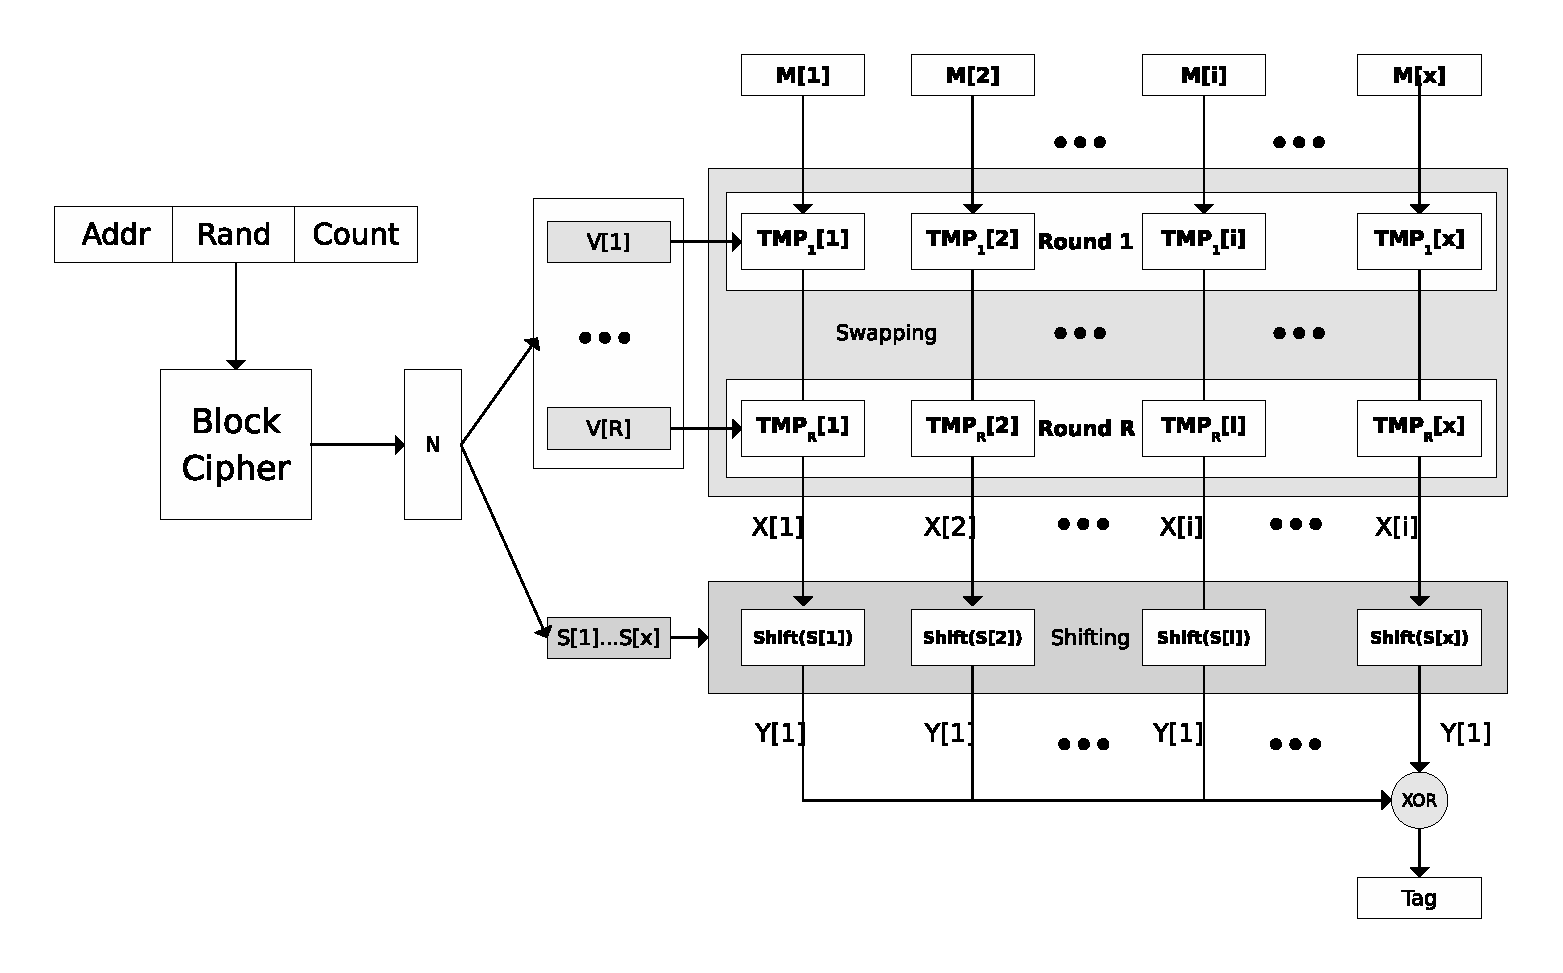
\includegraphics[scale=0.6]{./diagrams/CETD.eps}
 \caption{The CETD-MAC Scheme}
 \label{fig:CETD-MAC}
\end{figure}

\begin{figure}[htbp]
 \centering
 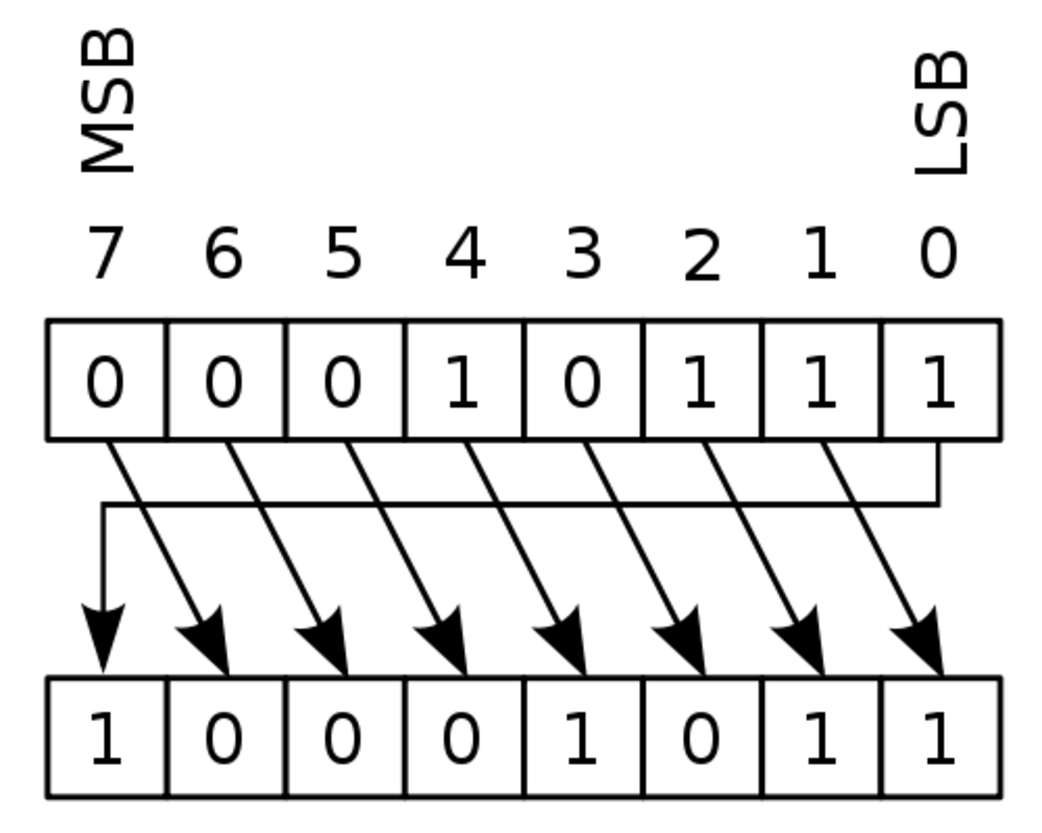
\includegraphics[scale=0.4]{./diagrams/rotate_right.pdf}
 \caption{The Concept of Rotate Shifting(Right)}
 \label{fig:rotate_shift}
\end{figure}
We follow the definition of CETD-MAC in \cite{keylist}. 
\begin{itemize}
	\item Message is splitted to sub-blocks each of whose length is tag length
	\item The first stage is several rounds of bit-segment swapping. For each round , two sub-blocks are randomly chosen. Introduce shuffle parameter V[i]
	\item The output sub-blocks from swapping stage, named X blocks, are sent to block-level rotate shifting stage. Each X block is rotate shifted for several bits. The concept of rotate shifting is expressed in Fig $\ref{fig:rotate_shift}$ Introduce shift parameter S[i]
	\item The output sub-blocks from shifting stage, named Y blocks, are XORed to form the final tag
\end{itemize}
Assume E$_K$ performance like a ideal random value generator, for two distinct nonce-inputs NI1 and NI2, the corresponding nonce values N1 and N2 should be random and the probability that N1 is identical to N2 should be 1/2$^n$, where n is Len(N1). 
%cetd can ensure that under copy-then-replay attack, the nonce input is distinct

%implent-level is secure
\paragraph{CETD meets the security requirement of CETD-MAC}
To defend copy-then-replay attack, CETD-MAC requires that when the chip writes
the content of a memory frame in an address, the nonce used to generate the tag
should be randomly chosen. As the nonce is generated by encrypting nonce-input,
the memory authentication system based on CETD-MAC should ensure that for each
time of memory writing, the nonce-input is distinct.

In CETD tag design, a input of nonce generation is a tuple(addr,ctr, rnd). The meaning of each element in the tuple is listed below: 
\begin{itemize}
	\item Addr: The address of ciphertext
	\item Ctr: A incrementing counter 
	\item Rnd: A random number
\end{itemize}
When the adversary replaces the memory frame with his copy frame from same
address but older time point, the counter part in the nonce-input of this copy
is smaller than the counter part in the nonce-input of the valid frame. This
difference of counter part ensure that the two nonce-inputs are distinct. 
On the other hand, when the adversary tries to replace the frame with a copy
from another memory address, the address part for two nonce-inputs will
different and the two nonce-inputs will be distinct.
We can see that Cost-Effective Tag Design can meet the security requirements of
CETD-MAC.

%in the design paper, the author assume the adversary can just do brute-force attack
\paragraph{CETD-MAC is secure under brute-force attack}
%in brute force attack, the adversary tries the tag one-by-one till passing
In \cite{}, the authors provided a security analysis of CETD-MAC scheme. The adversary is assumed to conduct brute force attack in which he randomly chooses a ciphtertext C and a nonce N. Then he keeps C and N fixed and tries different tags until a tag T can pass the verification with C and N. All the tags tried until passing the verification form a set named tag exploration space. The author assumed a MAC to be secure if the following conditions are met:
\begin{itemize}
	\item The size of tag exploration space is large
	\item If the ciphertext and nonce is randomly generated and unaccessible to the adversary, the probability to pass the verification for each tag in the tag exploration space is identical
\end{itemize}
Based the above two conditions, the author assume CETD-MAC is secure.

%security analysis based on computational definitions
\subsection{CETD-MAC is not PRF}\label{sect:proportion}
In this section we discuss the security of CETD-MAC under two tpyes of integrity attack.  The adversary is assumed to know the length of ciphertext and tag on the memory frame he acquired. 
We prove that the probability that the fake pair passes the verification scheme under both two attacks is determined by the proportion of the 1s and 0s in the input ciphertexts and provide the equations quantifying this relationship. This fact indicates that the adversary can choose special ciphertext-tag pairs which have higher probability to pass the verification compared with other pairs.  

%in this case nonce is fixed and serves as the key as the deterministic MAC schemes
%the number of queries to succeed a forgery attack can be at most 2^{n-1}
In the computational model based security analysis on MAC schemes, a secure MAC scheme should ensure that for any two input messages in the domain, the probability that their tags collide should be no more than an upper bound. This definition of secure MAC scheme is widely accepted and has been adopted in the security analysis of iterated MAC schemes such as CBC-MAC \cite{} and its variants \cite{}, and parallel MAC schemes such as PMAC \cite{} and its variants\cite{}. This definition emphasizes that when the key used in the MAC scheme is unaccessible to the adversary, the adversary cannot find any relationship between a given tag and a given input message. In the eyes of the adversary, a given tag can be generated by any message in the input domain and for a given input message, its tag can be any one value in the tag range. 
%chosen-message attack in spoofing scenario
\subsubsection{Content Modification Attack Scenario}
In this part we prove that for CETD-MAC, the input ciphertexts have relationship between their tags.  For a given tag, the number of possible inputs is limited and can be computed based on the tag value. On the other hand, for a give input ciphertext, the number of possible tag value is also limited and can be computed based on the ciphertext value. This fact indicates that when modifying the ciphertext part C1 of a memory frame, the number of possible ciphertexts C2 to replace C1 is limted. On the other hand, the adversary can manifast the fake ciphertext-tag pair C$_{fake}$-T$_{fake}$ based on the relanship between a ciphertext and its tag quantified in their part and win a much high probability to pass the verification stage compared with randomly choosing a ciphertext and a tag. 

When conducting content modification attack, the adversary modifies the content of a memory frame from (C, T) to (C1, T1). When the verification stage VF read the modified (C1, T1) pair, VF computes C1`s tag, marked as T$_{tmp}$, using the nonce N which is also used in computing T. If T$_{tmp}$ is identical to T1, then the content modification attack succeed. We can see that in content modification attack, for two pairs (C$_{origin}$, T$_{origin}$) and (C2, T1), their nonce N and N1 are identical. To succeed the content modification attack, the adversary will choose the C1 that has high probability to get tag value T    
%the properties of PRF
\paragraph{PRF in content modification scenrio}
We follow the analysis path in the security analysis of CBC-MAC from Bellare et
al \cite{}. The adversary is given a black box named oracle. There is a function
in the oracle which can be a MAC scheme or PRF and decided by coin flipping. The adversary has infinite
computational power and can choose any input sent to the oracle. If no matter
what kind of strategy that the adversary choose, he cannot tell which function
is in the oracle, we assume that the MAC scheme behaves like a PRF.  

As the tag space is limited, the tag value will repeat if the adversary call the
oracle too many times. However, the outputs from PRF have the following two
properties if the output space is large:
\begin{enumerate}
	\item All the element in the output space will appear
	\item The output values distribute uniformly and have no correlation. 
\end{enumerate}
Property 1 is the basic requirement of the functions that behave like PRF. One
counterexample that have property 1 but property 2 is a continuous counter.


\paragraph{The Diffusion Does Not Introduce New Bits}
In CETD-MAC scheme, the shuffle and shift stage relocate bits in the ciphertext to new index. Even though the new index of each bit in the cihpertext is unpredictble as the nonce is the output of a PRF and unaccessable to the adversary, it is certain the output of shift shuffle and shift stage contain same bits as the ciphertext. Assume ciphertext is consist of m blocks each of whose length is n bits, and there are totally k 1s in the m*n bits in the ciphertext. The the output of shuffle and shift stage also have k 1s and m*n - k 0s. 

%give Theorem of content modificatoin attack
\paragraph{The Number of Possible Tags for a Ciphertext is Limited}
\label{sect:bit-proportion}
If the MAC scheme is ideal and behaves like a PRF, for any input ciphertext, the probability that its tag equals to a specific value is 1/2$^n$, where n is Len(tag). 
As the both shuffle and shift subroutines in CETD-MAC scheme are diffusion operations, for each input ciphertext, its 0-1 proportion will be maintained until the xor subroutine. This fact means that for a specific input ciphertext, the number of its possible tag values is limited. For example, assume the input ciphertext is (0x0, 0x01) and the Len(tag) is 8 bits, we can see that there are only 8 possible values that CETD-MAC can producer with different nonce, which are {0x01, 0x02, 0x04, 0x08,0x10, 0x20, 0x40, 0x80}. The reason for this fact is that there are only a single '1' in the input ciphertext, which means the Y blocks that serve as the input of xor stage contain only a single '1', so it is impossible to produce tag values such as 0xFF or ohter ones containing more than one '1'. From this instance we can see that for a input ciphertext, as the shuffle and shift stage can not introduce new bits, so for any nonce value, the number of 0s and 1s in the blocks doing xor operation is always same as the proportion in the input ciphertext, which means the possible number of 1sx in the tag after the xor operation is limited. We summarize this fact to the Theorem $\ref{theo:tagNum-1s}$ and the proof is expressed in the appendix.
\begin{theorem}\label{theo:tagNum-1s}
Assume the input ciphertext of CETD-MAC scheme, marked as C,  is consist of m n-bits blocks and the nonce is a output from PRF. The number of possible distinct tag values, marked as num\_tag, is determined by the number of 1s, marked as k, in C. The relationship between num\_tag and k can be expressed as:
\begin{equation}\label{equ:tagNum-1s}
\begin{split}
num\_tag &= \sum_{i=0}^{\lfloor k/2 \rfloor} \binom{n}{k-2*i} if k \in [0,n)\\ 
		& =\sum_{i=0}^{\lfloor n/2 \rfloor} \binom{n}{n-2*i} if k \in [n,m*(n-1)]\\
		& = \sum_{i=0}^{(m*n-k)/2} \binom{n}{(m*n - k)-2*i} if k \in (m*(n-1),m*n] 	 
\end{split}
\end{equation}
\end{theorem}
Based on Theorem $\ref{theo:tagNum-1s}$ we get the Colloery $\ref{coro:odd-even}$ and $\ref{coro:max}$:
\begin{corollary} \label{coro:odd-even}
if there are even number of 1s in the input ciphertext of cetd-mac, then its tag will also contains even number of 1s; if there are odd number of 1s in the ciphertext, then its tag has odd number of 1s.
\end{corollary}
\begin{corollary} \label{coro:max}
For any input ciphertext, the size of its possible tag rage is no more than 2$^{n-1}$ where n is Len(tag).
\end{corollary}

The proof of Corollary $\ref{coro:odd-even}$ is provided in the appendix. 
From Theorem $\ref{theo:tagNum-1s}$ we can see that the domain of input ciphertext can be splitted into three groups based on the number of 1s. The rage size is identical to num\_tag. We can draw the following conclusion based on this fact:
\begin{itemize}
	\item the maximum value of num\_tag is 2$^{n-1}$ if k $\in$[n, m*(n-1)]. 
	\item The probability of tag collision is affected by the value of num\_tag
\end{itemize}
%a strategy for the adversary in spooofing scenario
\paragraph{Forgery Attack in Content Modification Scenario}
%Given a ciphertext and unknown nonce, the number of tags that a adversary needs to try is determined by the number of 1s in the ciphertext, this property can help the adversry contrive strategry to reduce the number of guessing.
%on the other hand, the adversary can deisgn its c-t pair according to this property. 
%besides same proportion ciphertext, what type of other ciphertext can the advesrary to use with high prob of passing?

In the computational based security analysis on MAC schemes, the behaviour of the adversary is modeled as probing valid ciphertext-tag pairs first then sending a forgery pair to the verification system. In content modification attack scenario this model can be depicted as that the adversary acquires a valid memory frame and try to modify the content. If the adversry knows the length of ciphertext and the tag, he will know the value of the ciphertext and the tag. 
As the input domain of CETD-MAC scheme can be splitted into groups leading to different tag ranges, the security definition of MAC schemes under content modification attack cannot be meet as the adversary can conduct the following two types of modification on the frame:
\begin{enumerate}
	\item Select a new ciphertext that has T$_{origin}$ in its possible tag domain. A better choice is to select a ciphertext with same number of 1s as the tag T$_{origin}$
	\item Replace the frame with a new pair (C2, T2) that T2 is in the possible tag domain of C2
\end{enumerate}
From Theorem $\ref{theo:tagNum-1s}$ we know that if the number of 1s in m*n bits is too large(more than m*(n-1)) or too small(less than n), the possible tag domain size is small. This fact means choosing a ciphertext from these two domains has high probability to pass the verification stage.

%chosen-message attack in replay scenario
\subsubsection{Copy-then-Replay Attack Scenario}
%input is fixed and the nonce changes for each query,
%the number of query

When conducting copy-then-replay, the adversary replace a valid memory frame with his stored copy of a frame from other address or same address but older time point. The probability that the adversary succeeds the copy-then-replay attack is determined by the probability that for a fixed input C, the two tags T1 and T2 are identical when their nonce N1 and N2 are randomly generated.

As depicted in Section $\ref{sect:bit-proportion}$, the 0-1 proportion of a ciphertext is maintained to the input blocks(Y blocks) of xor stage. This fact means for a fixed input, the Y block set Y1 and Y2 for two randomly generated nonce N1 and N2 have same 0-1 proportion.  
\paragraph{Forgery Attack on CETD-MAC in Copy-then-Replay Scenario}
From Theorem $\ref{theo:tagNum-1s}$ and its related Corollaries we an see that the proportion of the input ciphertext will determine the size of its tag range and the maximum tag range size if 2$^{n-1}$ which is acquired if the number of 1s in the input ciphertext is between n and m*(n-1).
This fact means if the input ciphertext replayed has too many or too little number of 1s, such as all 0s and all 1s ciphertext, the related tag range contains only one tag value: 0. That means no matter how random the nonce is, replaying all 0s and all 1s ciphertext will always succeed.

\subsection{CETD-MAC is not a Secure MAC}
In this part we prove that CETD-MAC is not a secure MAC. This assertion is made
based on the assertion that CETD-MAC is not a PRF.

%new MAC design based on CETD-MAC
\section{Security Improved CETD-MAC}
We have shown that the original CETD-MAC cannot effectively defend two types of integrity attacks as the number of distinct tags is determined by the proportion of 1s and 0s. In this section, we propose several approaches to improve the security of CETD-MAC. Firstly we tried to utilize the nonce and the operation existing in the original CETD-MAC design and then prove the reason that this attempt cannot succeed. Then we proposed our rationale on improvement based on the instruction from \cite{}.  
%we need to add gf-mult to provide no-linearity, gf-mult a nonce seg can do
%random inject together
%why cetd-mac is not secure
\subsection{Security Enhancement of CETD-MAC with Its Operations}\label{sect:pattern}
%it is impossible to modify cetd-mac with existing operations to enhance security
In this part we try to enhance the security of CETD-MAC without introducing new operations or data. We analyze the functionality of each operation first and discuss whether it is necessary to maintain each operation in the new design.
%why to add each operation, why insufficient to use each only ?
\subsubsection{Design Rationale of Original CETD-MAC Scheme}
CETD-MAC scheme is consist of three stages: bit-segment shuffle with user chosen shuffle round, then cycle shift for each output lf shuffle stage with randomly chosen shift length and finally xor all output block of shift stage to the tag. It is insecure to construct with only one of the three stages.
\paragraph{XOR stage}
The xor operation is a common choice for parallel MAC schemes to convert m n-bits block to a n-bits tag. It has been analyzed by Bellare in \cite{} that it is insecure to construct a MAC scheme with xor operation only as simply swapping the order of two blocks in the input can lead to tag collision.  The input blocks must be processed before sent to xor stage to ensure that simply changing the order of two input blocks in the input will change the input set of xor stage.
%shift is vulnerable to pattern
\paragraph{Cycle Shift Stage}
In original CETD-MAC scheme, cycle shift stage, short for shift stage, locates before the xor stage. For each input block of shift stage, the number of bits shifted is determined by the value of a nonce segment. Shift stage can defend the attacks such as changing the order of two input blocks as the adversary has no access to the nonce value and then can not predict the number of bits shifted of each block, then has no idea that changing the order of which two blocks lead to tag collision with high probability. However, it is still insecure to construct a MAC scheme by adopting shit stage then xor stage, as for some input blocks which are consist of one kind of patterns, shifting different number of bits can still lead to same output block. This fact means that reordering the blocks formed by a pattern have higher probability to lead to tag collision than other blocks. This fact is depicted in detail in Appendix $\ref{appendix:pattern}$. 

%why it is insufficient to use shuffle only if the number of blks are large?
\paragraph{Bit-Segment Shuffle Stage}
Shuffle stage swaps two bit-segments in each round. As the index and offset of swapping in each round is determined by the nonce, the adversary cannot predict which blocks participate the shuffle. One problem to use shuffle without shift is that if the number of blocks are large while the number of shuffle round is small, the number of blocks participating the shuffle is small. This fact is serious in copy-then-replay attack as majority of blocks may not participate shuffle and the content of these unshuffled blocks will be maintained until the next stage. %If the operation linked to shuffle is the xor stage directly without shift stage, according to Equation $\ref{}$ we can see that the probability of tag collision is determined by th

 In the original CETD-MAC, the shift stage will help re-ordering the bits in the output blocks from shuffle stage to ensure that the input blocks of xor stage is hard for the adversary to predict. 

 %diffusion is not enough
\subsubsection{Diffusion is insufficient to construct a secure MAC scheme}\label{par:diffusion}
%linearity analysis and different analysis
We can see what shuffle and shift do is reordering the bits in the input message
blocks. We give each input bit a index from 1 to m*n. When the nonce is fixed
and unknown, we are certain for two inputs M1 and M2 the bits with same index
will be relocated to same new index. The adversary does not know the exact bit
distribution of the input blocks to xor stage but he knows that the 0-1
proportion is same as the input of CETD-MAC. As depicted in Section $\ref{sect:proportion}$, the odd-even property of the tag is identical to its input, and the number of possible distinct tag values can be predict based on the number of 1s in the input. When realized this fact, the adversary just needs to choose a tag value that has same odd-even property and the number of 1s is no more than min(n,k), there k is the number of 1s in the input.

Content Modification Scenario
In content modification scenario, the adversary keeps modifying a memory frame in an address until the frame passes verification. The modification will be previous to the next write operation from the chip the same address. 

Copy-then-Replay Scenario
To eliminate this weakness, we need to add a operation to make sure that if the adversary does not know the value of the fixed nonce, he cannot predict the 0-1 proportion and bit distribution of the input blocks of xor stage. 
%we need no-linearity and rnd bits
\paragraph{No-linearity and Random Bit Injection}
In cite{},R and J depicted the design rationale of each operation in Rij AES. Their should be three types of operations in a block cipher design serving as no-linearity, random-bit injection and diffusion.  
In original CETD-MAC scheme, both shuffle and shift operation achieve the diffusion, while no operation can inject random bits for each input and all the operation in the CETD-MAC is linear.  
%block cipher consist of three operations
%no-linearity must be achieved with gf-mult

\paragraph{Galois Field Multiplication}
As mentioned in Section $\ref{par:diffusion}$, it is insufficient to use linear operation
only to construct a secure MAC scheme. The reason is that linear operations can
diffuse the bit distribution of the input while can not introduce new bits. On
the ther hand, the input and the output of linear operation has linear
relationship and the adversary can find the relationship and conduct successfule
forgery attack since then without acquiring the nonce or the key.

The we need to add no-linearity random bit injection operation. For the MAC
schemes constructed with block cipher, such as CBC-MAC(and its variants) and
PMAC(and its variants), the block cipher usually contains these two operations.
R and J mentioned in \cite{} the galois field multiplication and its inverse
operation can serve as no-linearity operation. 
For example in Rij AES, the ByteSub provide no-linearity to the input by
adopting the galois multiplication inverse to each input byte then affline
transformation with a constant matrix to the input. Random bits that stored in a
roundkey, which is acquired by expanding the encryption key, is injected to the
input by xoring the roundkey with processed input.  

In GMAC, the author utilized the galios field multiplication other than block
cipher to process each input block serially. Each input block does galois field
multiplication with H, which is acquired by encrypting constant 0 with a secret
key. The output of multiplication is xored with the next input block to serve as
the multiplicand for H. The advantage of multipling each xored input block with
H compared with calling the encryption function to the input block directly is
that the no-linearity and random bit injection is combined to one round
operation, which reduces the space cost and enhances the processing speed.

The application of GF multiplication in GMAC inspired us on the security
optimization of original CETD-MAC scheme as for each ciphertext to be processed,
a nonce is generated with block cipher. The nonce or its segment can serve as
the H in the GF multiplication in GMAC. 
%new designs
\subsection{Improved CETD-MAC with higher security level}
In this part we introduce our improved version of CETD-MAC. In our first attempt
of improvement, we do galois field multiplication, short for gf-mult, to each input block with a
segment extracted from nonce. We call this first attempt Fully-GFM CETD-MAC as
each input block will participate the galois mulatiplication. We also introduce
its variant named Selected-GFM CETD-MAC in which the number of input blocks
doing gf-mult is determined by user choice, just as what shuffle stage does. 

Adding gf-mult before shuffle can inject random bits to the inputs and the
adversary cannot predict the tag based on the input value according to the
attack strategry depicted in Section $\ref{sect:proportion}$. This improvement works for all
the input value except for all 0 input as the output of 0 gf-mult with any value
will be 0. To address this problem, we introduce our second version of improved
CETD-MAC scheme named Flip-then-GFM CETD-MAC scheme. We randomly flip each input
block and then do selecte gf-mult as we did in the variant of first version. We
will show that our second version of improved CETD-MAC is secure under two types
of integrity attacks in this part. 
%gf-mult only design
\subsubsection{Fully-GFM CETD-MAC}
Our first design draft based on the original CETD-MAC is named as Fully GF-Mult CETD-MAC, which mean each
input will do galois field multiplication with a nonce segment. The advantage of this draft is that if there is at least one bit value is identical to one in a input block, then the gf-mult on this block lead to an output block whose bit distribution cannot be predicted if the nonce segment is unaccessible. 
The are two disadvantages of this draft: firstly if a input block is all 0, then the gf-mult will generate all 0 output block no matter what nonce segment is applied; secondly a calling of gf-mult is much time costing compared with the shuffle or shift operation. 
\paragraph{Selected-GFM CETD-MAC}
As gf-mult is a time costing operation, for some embedded platform the high security brought the Fully GF-MULT CETD-MAC is less important as the update speed of the memory frame is high and the adversary has no enough time to finish the whole attack procedure. Base on this fact we modify the draft from conducting gf-mult on each input block to the new draft, which is named as Selected-GFM CETD-MAC. IN Selected-GFM, there is another input parameter r\_blk determine the number of input blocks which will be conducted gf-mult. Then r\_blk continuous input blocks will be selected and the index of first input block is determined by a segment on the nonce. 

Like Fully-GFM CETD-MAC, Selected-GFM CETD-MAC cannot process the all 0 input blocks either.
%flip-then-gf-mult
\subsubsection{Flip-then-GFM CETD-MAC}
As no matter fully or selected block version of GFM CETD-MAC, the input blocks consist of all 0s can not be processed as 0 gf-mult with any value will lead to 0. To address this  problem, we add another stage before selected gf-mult.
\paragraph{Block Flipping}
\paragraph{Flipping-GFM CETD-MAC}
%\renewcommand{\algorithmicrequire}{ \textbf{Input:}} %Use Input in the format of Algorithm
%\renewcommand{\algorithmicensure}{ \textbf{Output:}} %UseOutput in the format of Algorithm
%\begin{algorithm}[htb] 
%\caption{Fully Galois Field Multiplication} 
%\label{alg:fully-GFM} 
%\begin{algorithmic}[1] %这个1 表示每一行都显示数字
%\REQUIRE ~~\\ %算法的输入参数:Input
%The set of positive samples for current batch, $P_n$;\\
%The set of unlabelled samples for current batch, $U_n$;\\
%Ensemble of classifiers on former batches, $E_{n-1}$;
%\ENSURE ~~\\ %算法的输出:Output
%Ensemble of classifiers on the current batch, $E_n$;
%\STATE Extracting the set of reliable negative and/or positive samples $T_n$ from $U_n$ with help of $P_n$; 
%\label{ code:fram:extract }%对此行的标记,方便在文中引用算法的某个步骤
%\STATE Training ensemble of classifiers $E$ on $T_n \cup P_n$, with help of data in former batches; 
%\label{code:fram:trainbase}
%\STATE $E_n=E_{n-1}\cup E$; 
%\label{code:fram:add}
%\STATE Classifying samples in $U_n-T_n$ by $E_n$; 
%\label{code:fram:classify}
%\STATE Deleting some weak classifiers in $E_n$ so as to keep the capacity of $E_n$; 
%\label{code:fram:select}
%\RETURN $E_n$; %算法的返回值
%\FOR{each $i \in [1,9]$}
%\STATE initialize a tree $T_{i}$ with only a leaf (the root);\
%\STATE $T=T \cup T_{i};$\
%\ENDFOR
%\FORALL {$c$ such that $c \in RecentMBatch(E_{n-1})$} 
%\label{code:TrainBase:getc}
%\STATE $T=T \cup PosSample(c)$; 
%\label{code:TrainBase:pos}
%\ENDFOR
%\FOR{$i=1$; $i<n$; $i++$ }
%\STATE $//$ Your source here;
%\ENDFOR
%\FOR{$i=1$ to $n$}
%\STATE $//$ Your source here;
%\ENDFOR
%\STATE $//$ Reusing recent base classifiers. 
%\label{code:recentStart}
%\WHILE {$(|E_n| \leq L_1 )and( D \neq \phi)$}
%\STATE Selecting the most recent classifier $c_i$ from $D$;
%\STATE $D=D-c_i$;
%\STATE $E_n=E_n+c_i$;
%\ENDWHILE 
%\label{code:recentEnd}
%\end{algorithmic}
%\end{algorithm}


%\appendix
%\subsection{Security Theorem Proof}
%\subsubsection{Proof of Theorem $\ref{frequency-tag}$}

%\end{document}
